
% Author: PokMan Ho pok.ho19@imperial.ac.uk
% Script: LogisticTmp.tex
% Desc: `LaTex` report framework -- Logistic Growth
% Input: none
% Output: none
% Arguments: 0
% Date: Oct 2019

\documentclass[a4paper, 11pt]{article}
\usepackage[margin=1in]{geometry}
\usepackage{hyperref, setspace, lineno, amsmath, amssymb, longtable}
\usepackage{float} %% fix graphs at where they should be

%% test insert graphs
\usepackage{graphicx}
\graphicspath{ {../results/} } %% <https://www.overleaf.com/learn/latex/Inserting_Images>

%% test insert variables
\newcommand{\pml}{phenological model}
\newcommand{\pms}{phenological models}
\newcommand{\Pml}{Phenological model}
\newcommand{\Pms}{Phenological models}
\newcommand{\ReportTitle}{Microbial growth models -- which is better and why?} %% <https://stackoverflow.com/questions/1211888/is-there-any-way-i-can-define-a-variable-in-latex>
\newcommand{\ReportAuthor}{PokMan HO}
\newcommand{\ReportAffil}{Department of Life Sciences, Faculty of Natural Sciences,\\Imperial College London}
\newcommand{\Disclaim}{\textbf{A Mini-project submitted in partial fulfilment of the requirements for the degree of Master of Research at Imperial College London\\\\Formatted in the journal style of the \textit{Nature} Journal\\Submitted for the MRes in Computational Methods of Ecology and Evolution}}
\newcommand{\fve}{Verhulst (classical)}
\newcommand{\fgo}{modified Gompertz}
\newcommand{\fba}{Baranyi}
\newcommand{\fbu}{Buchanan}
\newcommand{\fqu}{quadratic}
\newcommand{\fcu}{cubic}
\newcommand{\pop}{population size}
\newcommand{\pps}{population sizes}

\title{\ReportTitle}
\author{\ReportAuthor\ (CID: 01786076)}
\date{}

%% citation
\usepackage[%
autocite    = superscript,
backend     = bibtex,
sortcites   = true,
style       = nature
]{biblatex}
\bibliography{../reference/Log_r.bib} %% <https://tex.stackexchange.com/questions/6805/bib-library-file-in-a-different-directory-how-to-use-mendeley-centralised-b>

%% set as required
\doublespacing
\linenumbers

\begin{document}
	\begin{center}
		\Huge\textbf{\ReportTitle}\\
		\LARGE\ReportAuthor\\
		\Large\ReportAffil
	\end{center}
	\begin{figure}[h]
		\centering
\includegraphics[width=\linewidth]{icl.jpg}
	\end{figure}
	\begin{flushright}
		\Large Approximate Word Count: %% insert approx word count
	\end{flushright}
	\clearpage
	
	\maketitle
	\section*{Abstract}
	
	
	\section*{Introduction}
	\Pms\ are expected to fit data trends within its biological field.  Yet due to different reasons, models developed and published from one sample may not fit the others.  These reasons may be due to data variabilities, confounding factors, inaccurate assumptions or models being too-specific.  This project is aimed at compare and contrast published \pms\ on microbial \pop\ data, highlighting which is a better model under what conditions.  The hypotheses are:
	\begin{itemize}
		\item published \pms\ are better than polynomials in describing microbial \pop;
		\item appropriate \pml(s) is/are identifiable through distinguishable shapes of microbial \pop; and
		\item parameters of data under each \pml\ is clustered, similar with dataset best-described by the same model but different from those described by other models.
	\end{itemize}
	
	\section*{Methods}
	Experimental microbial population growth data library were divided into individual data subsets through six filters (``Temperature (in $^o$C)", ``Microbial clade", ``growth substrate materials", ``experimental replicate number", ``population data recording unit" and ``data source").  Records with data unit ``OD\_595" were scaled into optical density percentages (i.e. data*100) to facilitate general analyses workflow.  Independent (or explanatory) variable was ``Time (hr)" and dependent (or response) variable was ``\pop".\\
	Some raw data were recorded in minutes (instead of hour).  This record artifact was not corrected because of two reasons: 1. shape of curves were the main concern instead of independent variable's scale; and 2. the unit was consistent within each data subset.
	
	\subsection*{Model assessment}
	Six candidate models were assessed, four phenological and two polynomial equations.  They were ``\fve"\autocite{mckendrick1912xlv}, ``\fgo"\autocite{GIL200689}, ``\fba"\autocite{baranyi1993modeling}, ``\fbu"\autocite{buchanan1993differentiation}, ``\fqu" and ``\fcu". Non-linear least square (NLLS) approach was used only on the four \pms\ and linear model-fitting was done on the two polynomials.  Starting values selection (for \pms\ only) was described below:\\
	Initial (N0) and final (K) \pps\ were selected to be the minimum and maximum values of each data subset respectively.  Maximum growth rate (r.max) was selected by linear model through a recursive manner.  For every iteration, \pop\ data from the top 5\% independent variable values were excluded from the linear model calculation.  The data and slope would only be recorded if it was positive, higher adjusted R$^{2}$ value and larger slope than the recorded ``best slope" value.  After scanning from the maximum side, the best slope and its respective data were taken out and screened from the minimum side.  Final best slope and x-intercept were regarded as the r.max and relative time lag (t.lag) of the population (in the source experiment) respectively.  Time which this linear model intersected with K was regarded as the time achieving carrying capacity (t.K).  Population data was then classified into three groups (gx) according to the time: g1 $\leq$ t.lag $<$ g2 $<$ t.K $\leq$ g3.  5\% was chosen as the scanning threshold because the author assumed this resolution was fine enough for achieving good starting values for NLLS fitting.  Inputs for \pms were listed below (popn \& time were the dependent and independent variables respectively):\\
	\begin{tabular}{rl}
		\fve: & popn = $f$(N0, K, r.max, time)\\
		\fgo: & popn = $f$(N0, K, r.max, time, t.lag)\\
		\fba: & popn = $f$(N0, K, r.max, time, t.lag)\\
		\fbu: & popn = $f$(N0, K, r.max, time, t.lag, gx)
	\end{tabular}\\
	
	All test starting values were than sampled from normal distribution with mean as the estimated value and standard deviation (sd) of 1.  The sd value was chosen because of different reasons for each parameters.  N0 and K were directly extracted from the raw experimental data, which could be assumed being an accurate estimate for that data subset (hence a small sd was logical). r.max was a guesstimated value from fitting linear models.  This process could potentially be affected by extreme values in the data and hence a large sd should be preferred.  100 trials were done as a optimal value under a trade-off between efficiency and accuracy.\\
	
	Only AIC\autocite{johnson2004model,akaike1998information,burnhamdr} was used to select for optimal parameter values within each \pml\ and best model between the six candidates for a data subset.  Reasons would be listed in Discussion section.  For models with more than one parameter sets as sharing the lowest AIC value, the first set of values from the random sampling trials were used for Kruskal-Wallis analysis.  All the available parameter sets were used to principal component analysis (PCA).  AIC tolerance threshold was expanded to min(AIC)+2\autocite{burnham2004multimodel} to incorporate more accepted models for analyses.
	
	\subsection*{Statistical analysis}
	Kruskal test was used for identify the best-fit model among all included model because the count was categorical and not assumed being normally-distributed.  Pairwise Nemenyi comparisons would be carried out to identify the best test if p-value of the above test was significant.\\
	
	Using PCA, parameter weights could be observed across \pms.  All parameter values met the ``minimal AIC +2"\autocite{burnham2004multimodel} criteria were extracted.  The t.lag values for datasets calling \fve\ as ``best-fit" were set zero (as this model do not need this parameter).  With datasets as rows, R-way analysis was done after all parameter data was natural-logged.  \Pms\ would be positively-correlating with a parameter if dataset observations were concentrated towards the positive side of the factor and vice versa.  It was expected that datasets would cluster together (or being on similar positions) if parameter(s) were representing the observed data.\\
	
	After that, all data used in the PCA analysis were analysed by individual factor (i.e. N0, K, r.max and t.lag).  This was done by Kruskal-Wallis test.  The data would be also analysed using post-hoc Tukey pairwise comparison if the Kruskal test showed significance.
	
	\subsection*{Main Assumptions}
	\begin{itemize}
		\item there was no negative population growth (i.e. starting population was always lower than carrying capacity), so negative population growth data were set to zeros;
		\item estimated parameter estimates would always result in a global optimal status in parameter space through the NLLS method.
	\end{itemize}
	
	\subsection*{Computing tools}
	R (ver 3.6.0)\autocite{Rcore} was used with ``minpack.lm"\autocite{minpacklm} for computing non-linear least square statistics for model comparisons.  ``stats"\autocite{Rcore} was used for Kruskal test and PCA analysis.  ``PMCMR"\autocite{PMCMR} was used for carrying out Nemenyi post-hoc pairwise comparisons for Kruskal test when needed.
	
	\section*{Results}
	\begin{figure}[H]
		\centering
		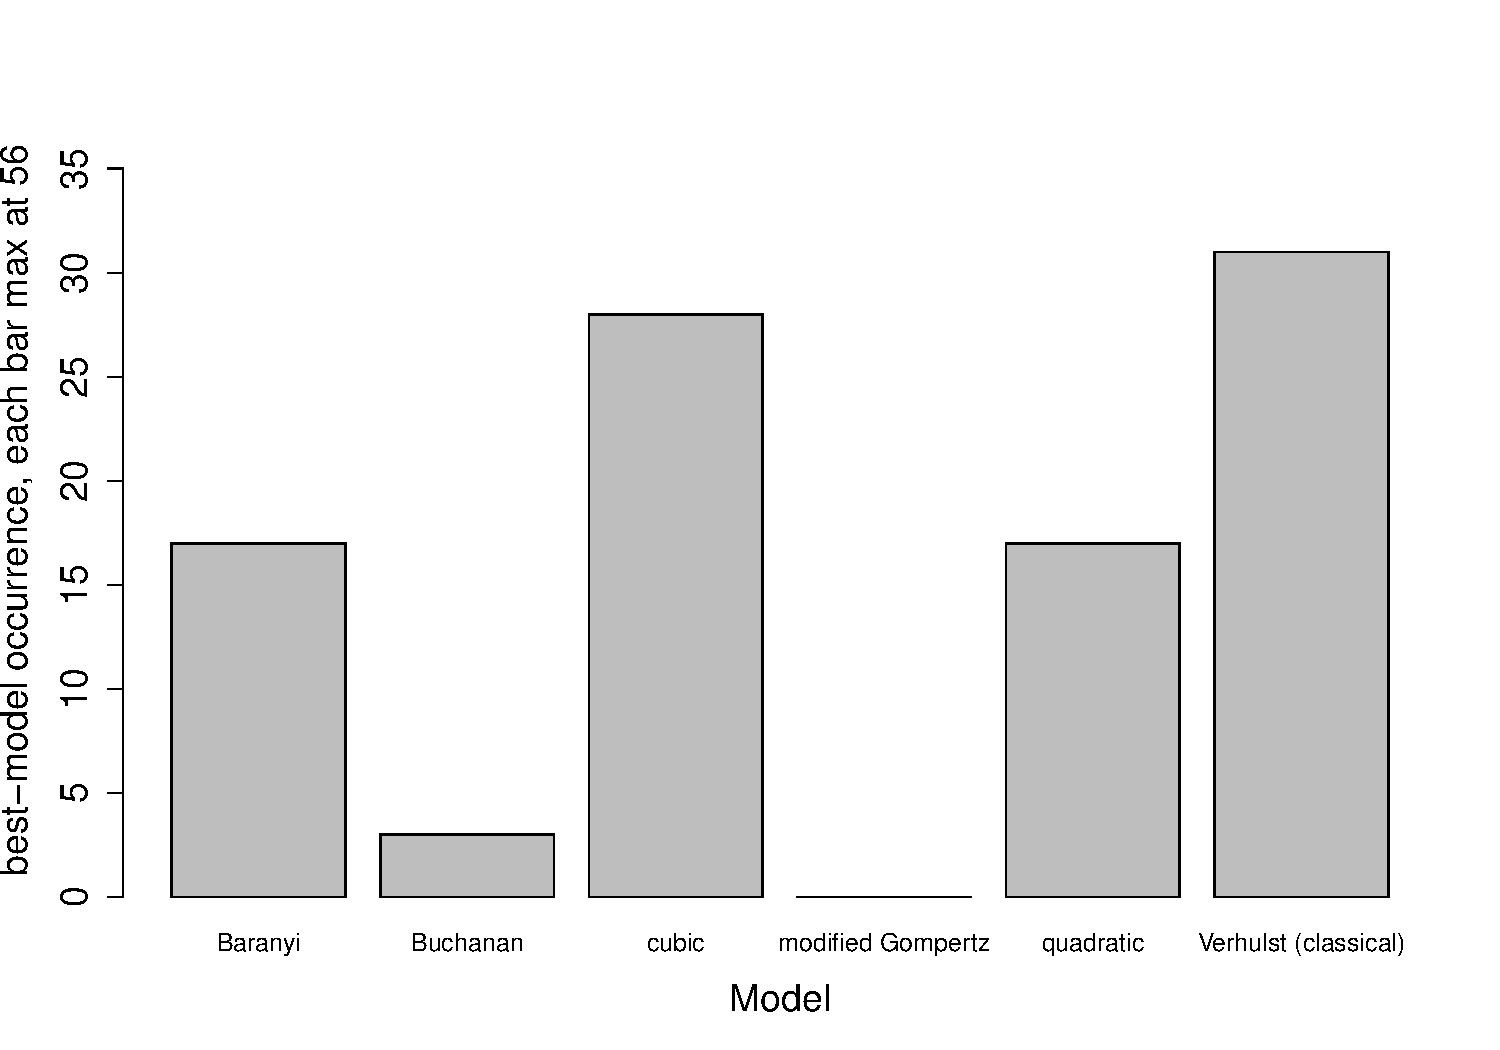
\includegraphics[width=.8\linewidth]{../results/barplot_BestModel.pdf}
		\caption{Barplot showing the number of ``best model" identification under AIC model-selection methods with ``
			%%insert_num_here
			" statistic $X^{2}$ = 
			%% insert_num_here
			, df = 
			%% insert_num_here
			, p = 
			%% insert_num_here
		}\label{barPT}
	\end{figure}
	From Fig.\ref{barPT}, large fluctuations between each model to be described as ``best-fit" were observed.  However the occurrence difference was not statistical significant.  Among the counts, there were 
	%% insert_num_here
	datasets with more than one ``best-fit" models.  \fve\ and \fcu\ were the top two models selected as ``best-fit" for the 
	%% insert_num_here
	 datasets (
	 %%insert_num_here
	  for \fve\ and 
	 %% insert_num_here
	  for \fcu
	 ).  There are 
	 %% insert_num_here
	  datasets calling both ``best-fit" at the same trial.  Between \fba\ and \fqu, the counts were 
	 %%insert_num_here
	  and 
	 %%insert_num_here
	  respectively with 
	 %% insert_num_here
	 datasets calling both models ``best-fit".  The only outstanding performance was from \fgo, which 
	 %% insert_num_here
	  datasets were called it as ``best-fit".\\
	  
	 \begin{figure}[H]
	 	\centering
	 	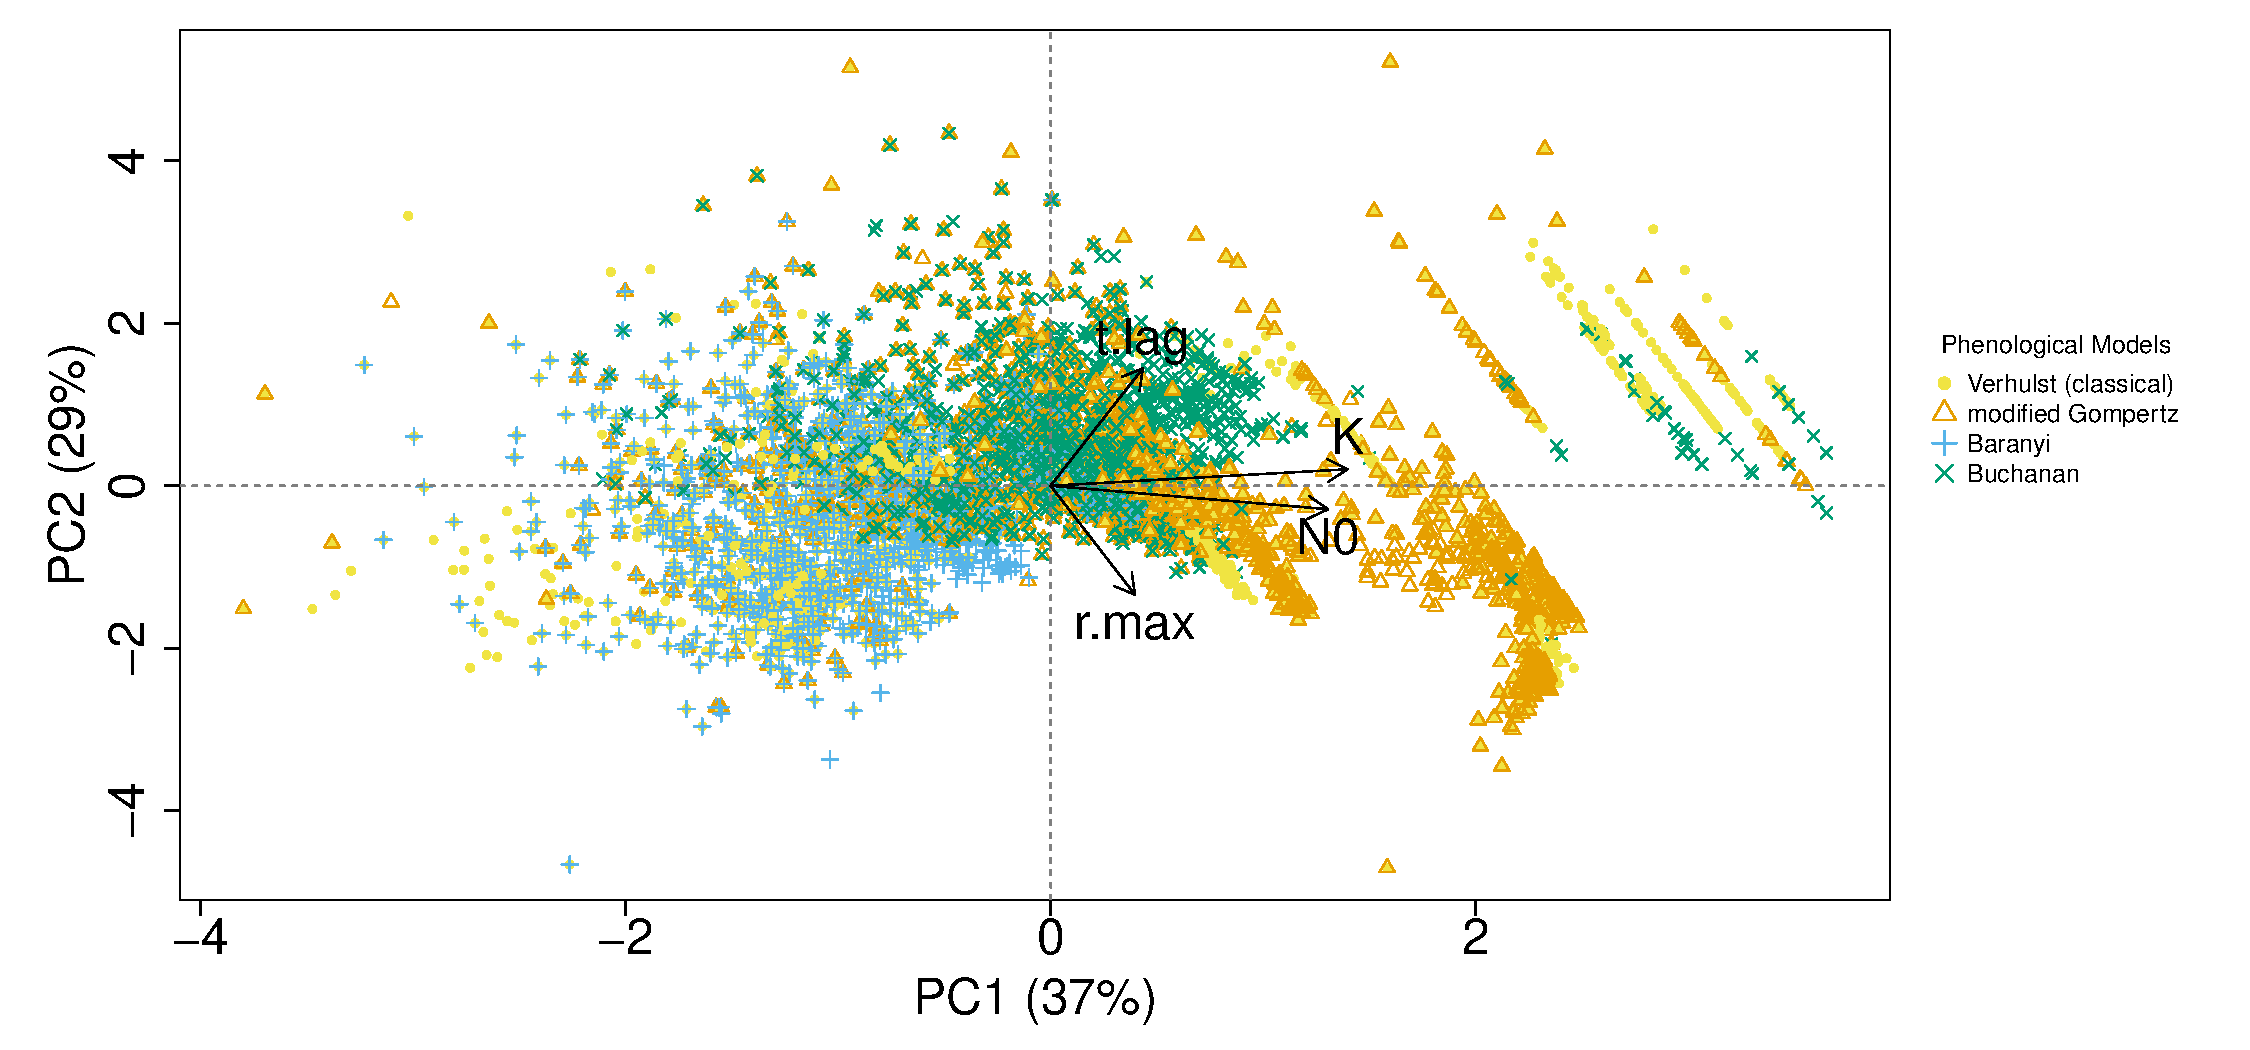
\includegraphics[width=\linewidth]{../results/Log_PCA.pdf}
	 	\caption{Biplot of Principal Component Analysis (PCA) comparing \pms\ using estimated parameter values with ``minimal AIC +2"\autocite{burnham2004multimodel} evaluations.}\label{biptPCA}
	 \end{figure}
 \begin{figure}[H]
 	\centering
 	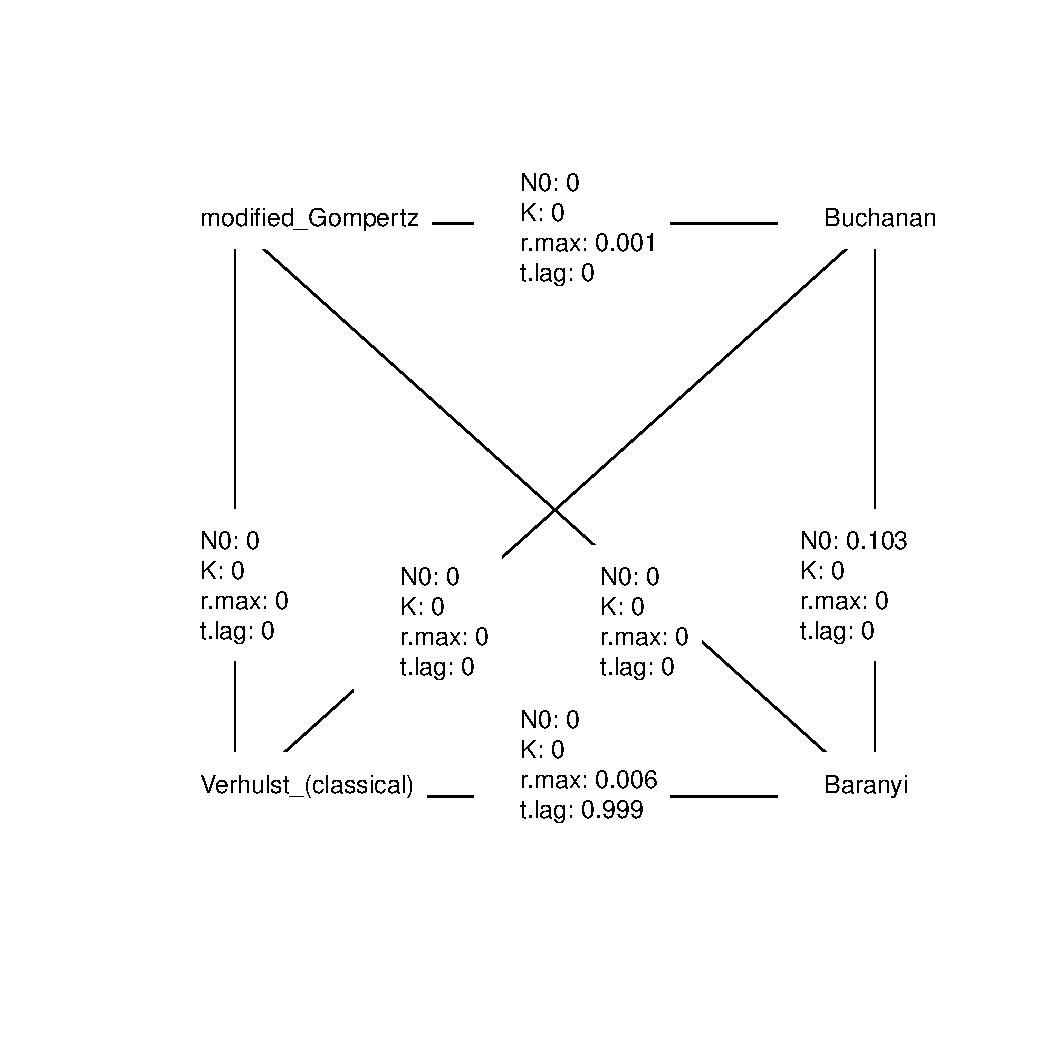
\includegraphics[width=\linewidth]{../results/Log_PCA_kt.pdf}
 	\caption{P-value summary between models on the four parameters under post-hoc Tukey-Dist pairwise comparison from Kruskal-Wallis Test.  Kruskal tests for all four factors were significant (
 		%% insert_num_here
 		: $X^{2}$ =
 		%% insert_num_here
 		, df = 
 		%% insert_num_here
 		, p-value = 
 		%% insert_num_here
 		; 
 		%% insert_num_here
 		: $X^{2}$ =
 		%% insert_num_here
 		, df = 
 		%% insert_num_here
 		, p-value = 
 		%% insert_num_here
 		; 
 		%% insert_num_here
 		: $X^{2}$ =
 		%% insert_num_here
 		, df = 
 		%% insert_num_here
 		, p-value = 
 		%% insert_num_here
 		; 
 		%% insert_num_here
 		: $X^{2}$ =
 		%% insert_num_here
 		, df = 
 		%% insert_num_here
 		, p-value = 
 		%% insert_num_here
 		).}\label{pValDraw}
 \end{figure}
 \begin{figure}[H]
	\centering
	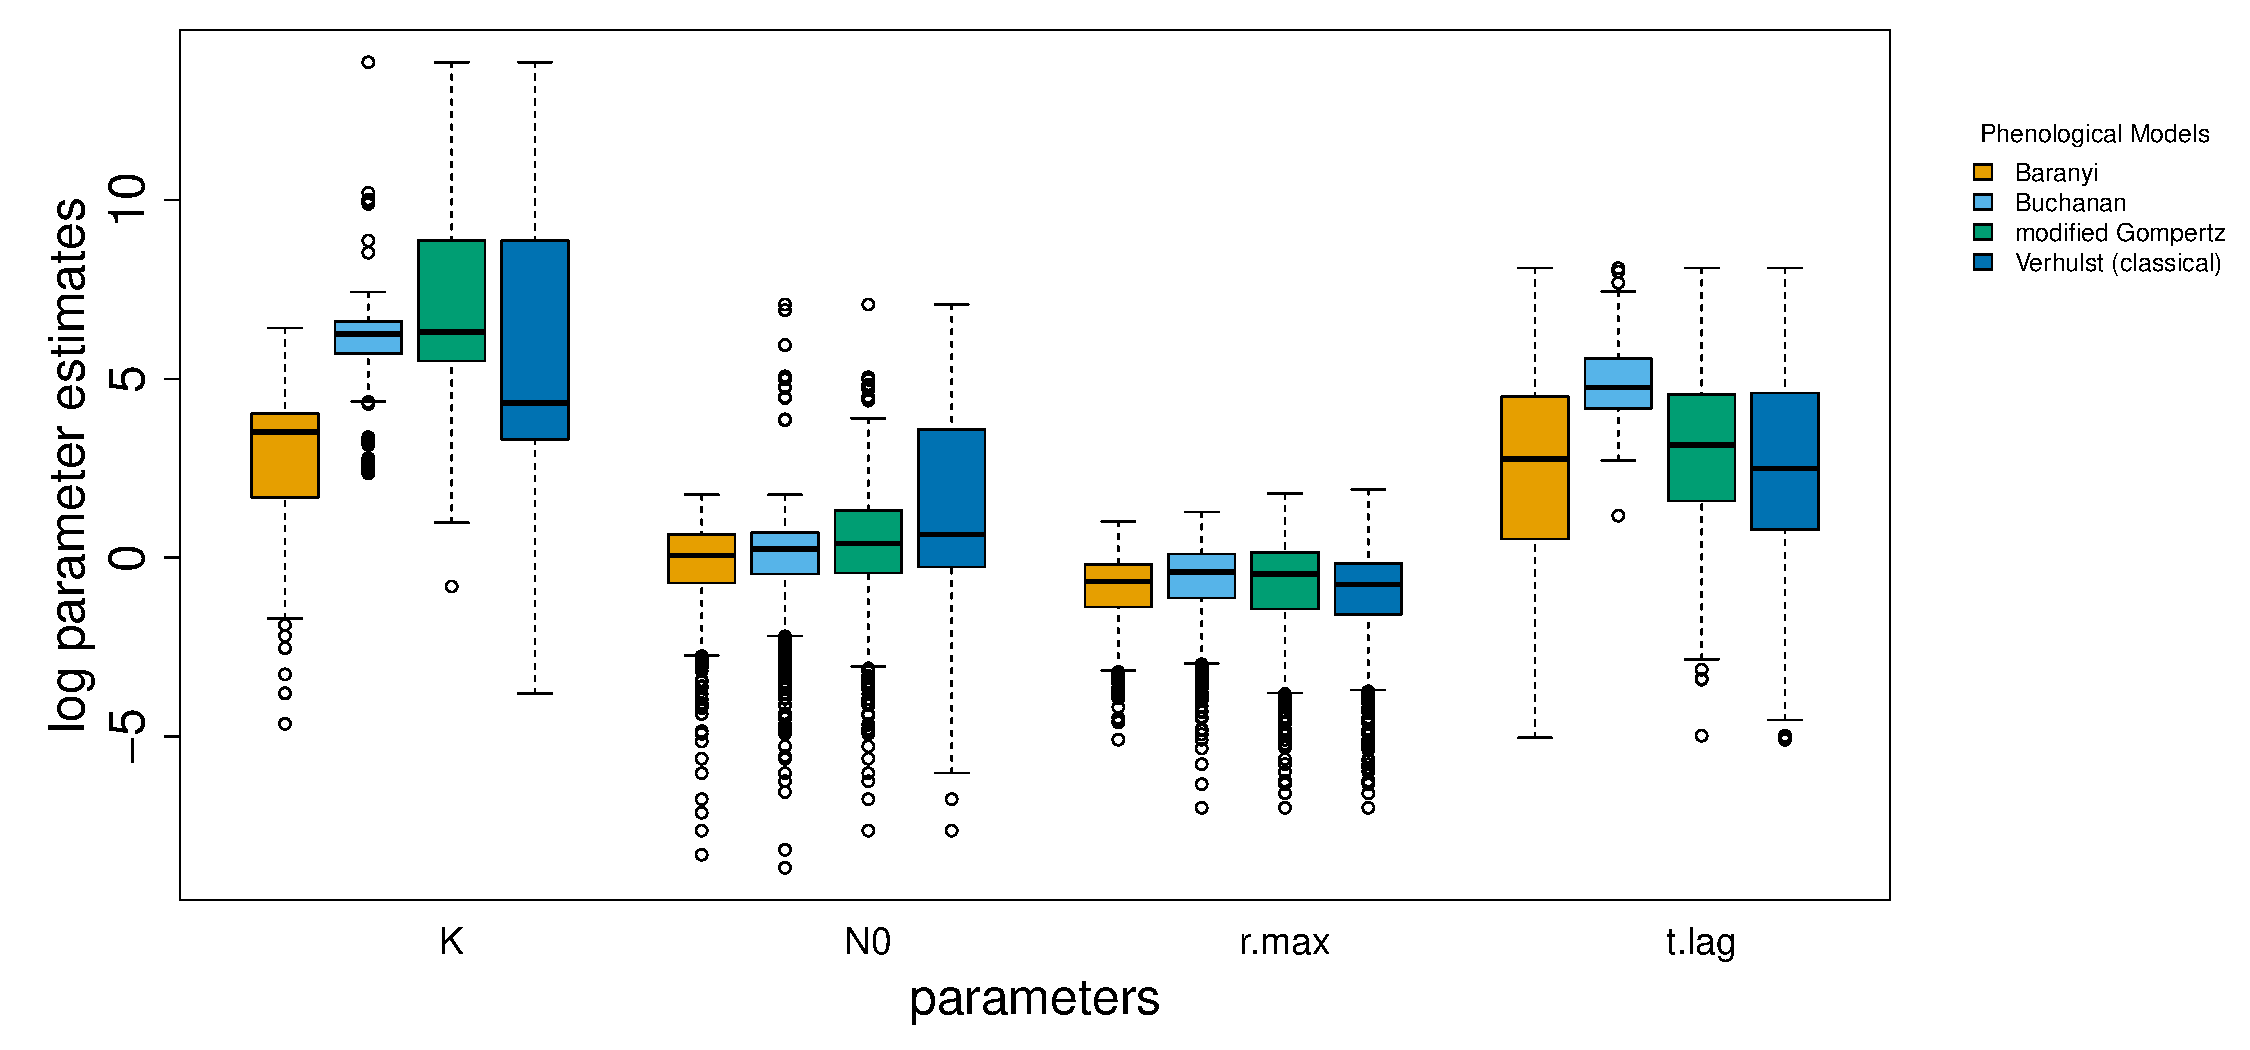
\includegraphics[width=\linewidth]{../results/Log_boxPerFac.pdf}
	\caption{Boxplot of log parameter values grouped by \pms.  Statistical results were summarized in Fig.\ref{pValDraw}}
\end{figure}
 In Fig.\ref{biptPCA}, principal component 1 (PC1) was capturing 
 %% insert_num_here
 \% variability.  It was composed approximately by 
 %% insert_num_here
  N0, 
 %%insert_num_here
  K, 
 %% insert_num_here
  r.max and 
 %% insert_num_here
  t.lag.  PC2 was capturing 
  %%insert_num_here
  \% variability.  It was composed approximately by 
 %% insert_num_here
  N0, 
 %%insert_num_here
  K, 
 %% insert_num_here
  r.max and 
 %% insert_num_here
  t.lag.\\
 
 There were 
 %% insert_num_here
  datasets with \pms\ fitting, although they may not be the ``best-fit" ones.  Datasets 
 %% insert_num_here
  were strictly limited to polynomial-fitting (Fig.\ref{lineOut}).  Among the \pms fitting datasets, \fve\ was the umbrella function, which can be fitted to most \pml-friendly datasets.
 \begin{figure}[H]
 	\centering
 	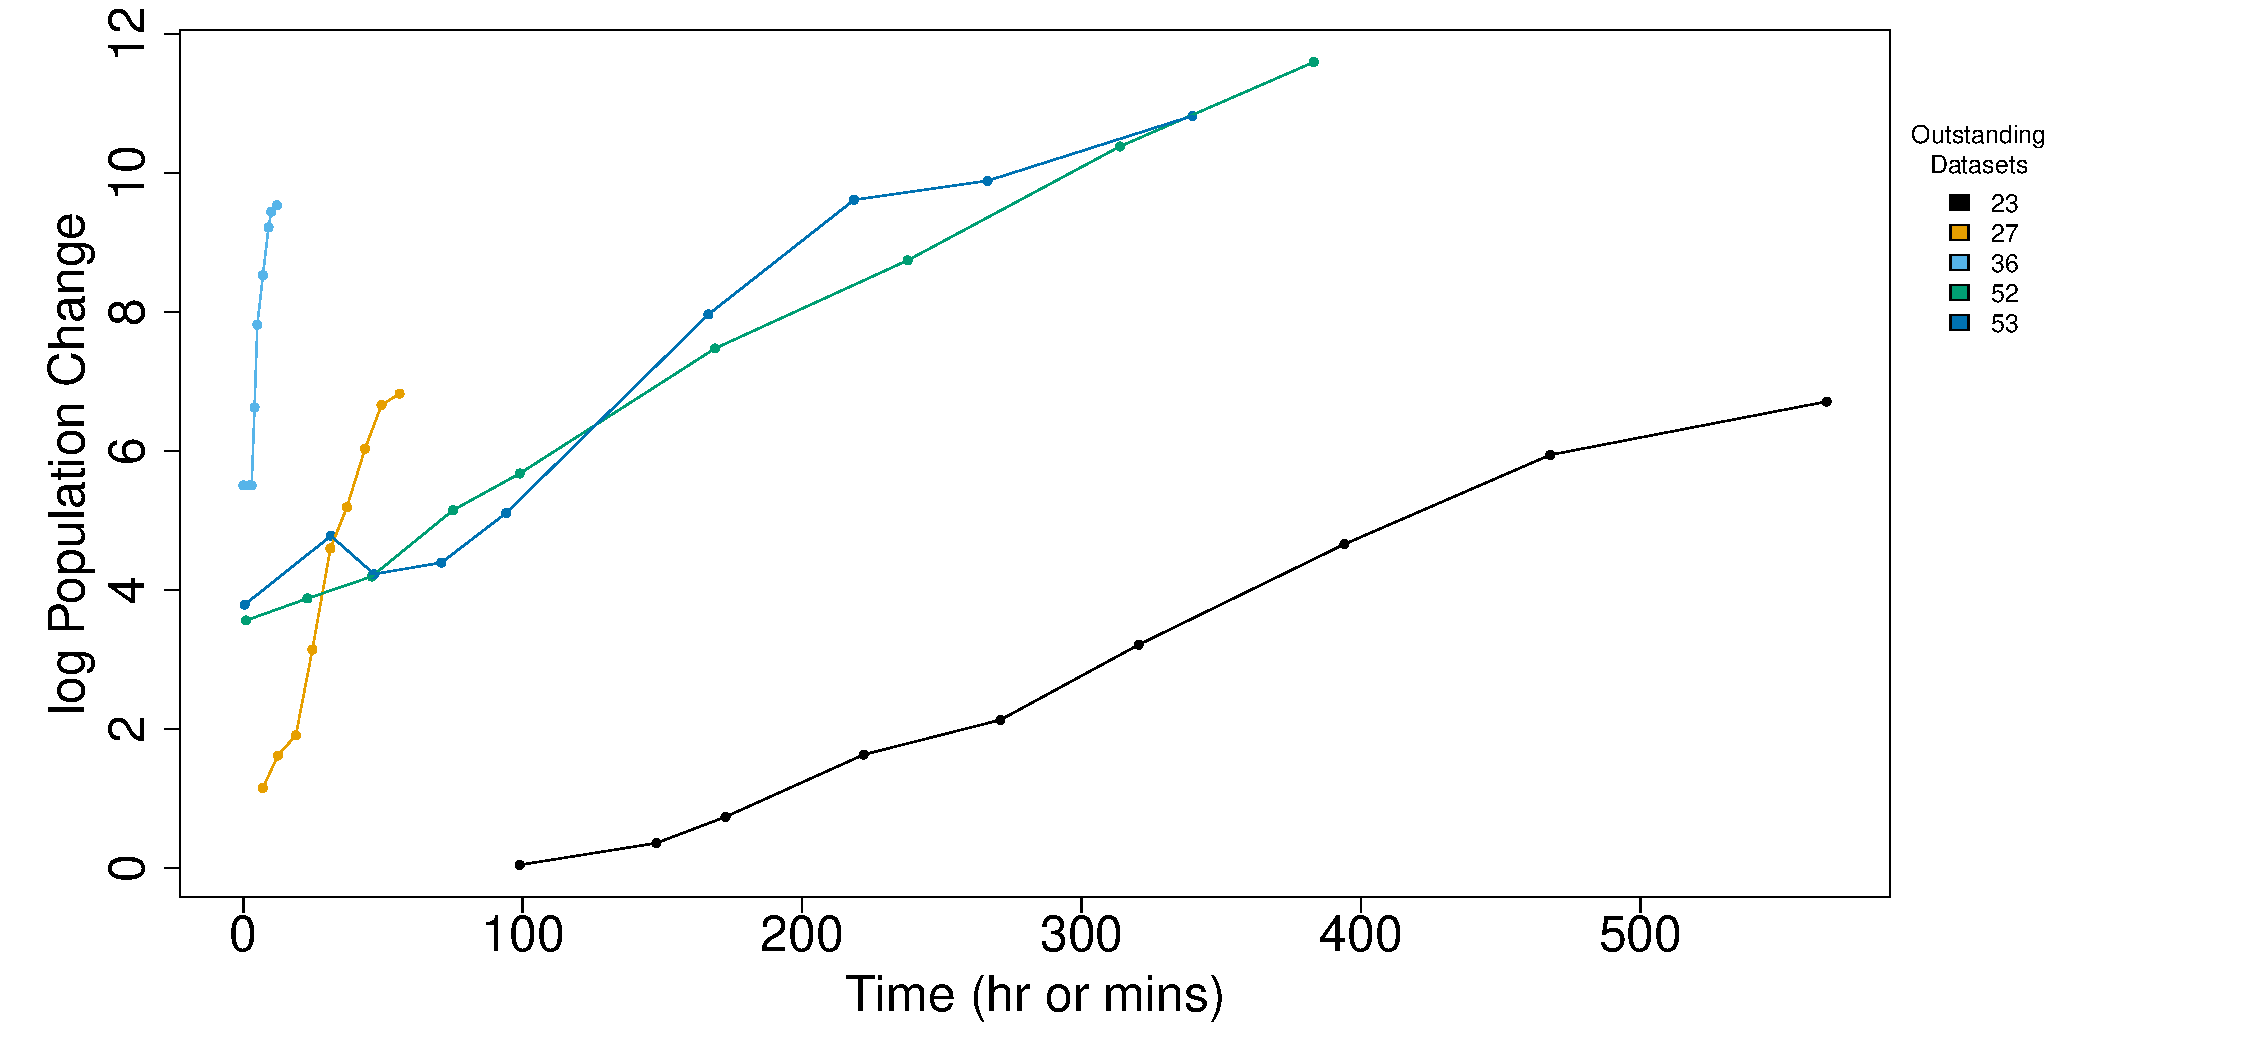
\includegraphics[width=\linewidth]{../results/Log_outstanding.pdf}
 	\caption{Line plot of datasets restricted to polynomial fits.}\label{lineOut}
 \end{figure}
From Fig.\ref{biptPCA}, \fve\ was having the widest coverage across parameter space.  However it did not have specific inclination towards any factors.  All other three models (\fgo, \fba\ and \fbu) were generally modelling subsets of the \fve\ coverage.  \fgo\ was able to model most of the data covered by the \fve.  Yet a larger successful trials were towards positive responses for N0, K and r.max.  \fba\ was a more specific model better in describing datasets with negative responses towards all parameter factors except r.max.  \fbu\ was having similar specificity comparing with \fba.  Datasets describable by this model were generally neutral responses towards all four parameters.  No models were found well-describing datasets positively correlating with t.lag while negative correlating with r.max.
	
	\section*{Discussion}
	%% AIC vs BIC <https://www.methodology.psu.edu/resources/AIC-vs-BIC/>
	%% AIC <https://en.wikipedia.org/wiki/Akaike_information_criterion#Comparison_with_BIC>
	%% BIC <https://en.wikipedia.org/wiki/Bayesian_information_criterion>
	%Model fitness to real data and simplistic mathematics were favoured by both AIC\autocite{johnson2004model,akaike1998information,burnhamdr} and BIC\autocite{johnson2004model,turchin2003complex}.  Apart from that, BIC also takes account of sample size effect\autocite{johnson2004model,turchin2003complex}.\\
	%comparisons in different fields\autocite{kuha2004aic,aho2014model,yang2005can,vrieze2012model,wang2006comparison,acquah2010comparison}\\
	
	AIC is considered the most suitable model-selection approach within model and between models in this project.  Unlike BIC, AIC are more accurate with small sample sizes\autocite{acquah2010comparison,kuha2004aic} and sparse data\autocite{kuha2004aic}.  AIC did not assume a ``true model" was under examination\autocite{aho2014model,vrieze2012model,yang2005can}.  Since candidate models were not ``nested model", BIC is not a better choice than AIC\autocite{wang2006comparison}.  Hence the use of only AIC as model-selection criterion should be justified.\\
	
	Although \fba\ and \fbu\ were observed occupying different parameter space (Fig.\ref{biptPCA}), these differences were not statistical significant (Fig.\ref{barPT}).
	
	\section*{Conclusion}
	Published \pms\ were data-specific, which none of them were found significantly performing better than the others in general.  Parameters defined by these \pms\ were appropriate, which none of them were having observable domination nor negligible weights on the function calculations.  There were assumptions embedded within the \pms\ which have limited its ability to describe data without a distinct sigmoid shape.
	
	\section*{Code and Data Availability}
	All \href{https://github.com/ph-u/CMEECourseWork_pmH/tree/master/MiniProject/code}{scripts} and \href{https://github.com/ph-u/CMEECourseWork_pmH/tree/master/MiniProject/data}{data} used for this report were publicity available at GitHub.
	\nocite{*}\printbibliography
	
	\section*{Appendix}
\begin{table}
		\caption{Table showing dataset id details for Fig.\ref{lineOut}}\label{table:source}
	\begin{tabular}{l|llllll}
		id&Temp ($^{o}$C)&clade&substrate&replicate&Source&Pop unit\\\hline
		%% insert_num_here
	\end{tabular}\\
	``Source" column publication key:\\
\begin{longtable}{p{.05\linewidth}p{.9\linewidth}}
	%% insert_num_here
	%% insert_num_here
	%% insert_num_here
	%% insert_num_here
	%% insert_num_here
	%% insert_num_here
	%% insert_num_here
	%% insert_num_here
	%% insert_num_here
	%% insert_num_here
\end{longtable}
\end{table}

\end{document}
